\thispagestyle{empty} % нет номеров страниц
\begin{minipage}{.3\textwidth}
    \vspace{-2cm}
    \textbf{M262.}
    \textit{Какое наибольшее число} а) \textit{ладей}, б) \textit{ферзей можно расставить на шахматной доске }8$\times$8\textit{ так, чтобы каждая из этих фигур была под ударом не более, чем одной из остальных?}
    \begin{flushleft}
        \vspace{0.5cm}
        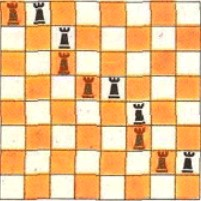
\includegraphics[width=\textwidth]{images/1.png}
        \captionof{Рис. 8}{ }
        \label{fig:8}
        
        \vspace{0.5cm}
        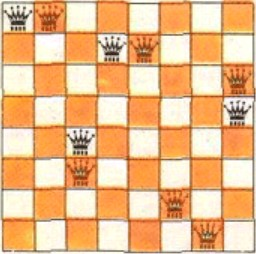
\includegraphics[width=\textwidth]{images/2.png}
        \captionof{Рис. 9}{ }
        \label{fig:9}
    \end{flushleft}

    \vspace{2cm}
    \textbf{M263.}
    \textit{Даны два числа p и q, большие 1. На сторонах BC и DC прямоугольника $ABCD$ берутся точки P и Q так, что $|BC| = p$. $|BP|$ и $|DC| = q$. $|DQ|$. При каком отношении длин сторон AB и AD угол $PAQ$ будет иметь наибольшую величину? Какова эта наибольшая величина в частном случае p = 2, $q = \frac{3}{2}$?}
\end{minipage}
\hspace{0.5cm}
\begin{minipage}{.6\textwidth}
   \hspace{0.5cm}Следуя письму \textit{Бориса} и \textit{Льва Рабиновичей}, предложивших эту задачу, рассмотрим сразу доску размером $n\times n$ и докажем, что на ней нельзя расставить более $\frac{4n}{3}$ ладей так, как требуется в условии.
    
    \hspace{0.5cm}Пусть $k$ ладей расположены на доске  $n\times n$ с соблюдением условия. На каждом поле, где стоит ладья, напишем число 0. В каждом из $n$ столбцов проделаем следующую операцию: если в столбце стоят два числа, то прибавим к обоим по 1, если одно число, то к нему прибавим 2 (в пустом столбце ничего писать не будем). Затем проделаем такую же операцию с каждой строкой. Ясно, что на месте каждой из $k$ ладей в результате будет написано число не меньшее 3~--- а именно либо 3, либо 4, --- поэтому сумма $S$ всех написаннных чисел не меньше $3k$; с другой стороны, поскольку в каждый из $n$ стобцов и затем в каждую из $n$ строк мы добавили не более чем 2, то сумма $S$ не больше $4n$. Итак, $3k\le4n$, откуда $k\le\frac{4n}{3}$

    \hspace{0.5cm}В частности, для $n=8$ получаем $k<\frac{32}{3}$, то есть $k\leq10$. Пример расстановки 10 ладей, удовлетворяющей условию, показан на рисунке 8.

    \hspace{0.5cm}Нетрудно проверить, что для любого натурального $n$ тем же самым способом можно на доске $n\times n$ расставить $[\frac{4n}{3}]$ ладей c соблюдением условия ($[x]$ означает целую часть числа $x$). 
    
    \hspace{0.5cm}Перейдём к задаче о расстановке ферзей. Ясно, что с собюдением условия задачи ферзей можно поставить не больше, чем ладей. На рисунке 9 показано, что на доске $8\times 8$ можно расставить 10 ферзей. Итак, в обих задачках а) и б) ответ одинаковый: 10.

    \hspace{0.5cm}Что же касается обобщения задачи Рабиновичей о расстановке ф е р з е й для доски $n\times n$, то её полностью не решил никто из читателей. Можно убедиться, что для $n=3,4,5$ наибольшее число ферзей, которое можно расставить на доске $n\times n$ так, чтобы каждый попал не более чем под один удар, на единицу м е н ь ш е $[\frac{4n}{3}]$. Но для больших n решение задачи требует, по-видимому, либо очень \emph{большого количества вариантов, либо привлечения дополнительных соображений.}
    \begin{flushright}
        \textsl{H.Б.Васильев}
    \end{flushright}

   \hspace{0.5cm}Обозначим длины сторон прямоугольника $AB$ и $AD$ через $a$ и $b$ соответственно. Тогда 
   
   $\tg(\angle PAQ)=\frac{\tg(\angle PAD)-\tg(\angle QAD)}{1 + \tg(\angle PAD)\cdot\tg(\angle QAD)}=$
   
   \begin{flushright}
        \Large{$\approx\frac{\frac{ap}{b}-\frac{a}{qb}}{1+\frac{a^2p}{b^2q}}=\frac{ab(pq-1)}{a^2p+b^2q}$}.
   \end{flushright}
  В силу теоремы о среднем арифметическом и среднем геометрическом, имеем

  \begin{center}
      $a^2p+b^2q\ge2\sqrt{a^2pb^2q}=2ab\sqrt{pq}$
  \end{center}
  (знак равенства имеет место при $a^2p=b^2q$, то есть когда
  \begin{center}
      \large{$\frac{a}{b}=\sqrt{\frac{q}{p}}\Big)$}.
  \end{center}
\end{minipage}